\section{Results}

% TODO: Formatting.
\subsection{Delta Method}
\begin{table}
    \begin{tabular}{l|lll}
        \textbf{Opponents} & \textbf{PAN 2013 Test 1} & \textbf{PAN 2013 Test 2}
        & \textbf{PAN 2015 Test} \\ \hline
        1  & 0.58685 & 0.58283 & 0.55870 \\
        2  & 0.62235 & 0.60125 & \textbf{0.56550} \\
        3  & 0.63348 & 0.60771 & 0.53969 \\
        4  & 0.63741 & 0.62173 & 0.52880 \\
        5  & 0.63483 & 0.61897 & 0.52269 \\
        6  & 0.63876 & 0.62787 & 0.52080 \\
        7  & 0.64337 & 0.63188 & 0.51399 \\
        8  & 0.64123 & 0.63488 & 0.51270 \\
        9  & \textbf{0.64438} & 0.63173 & 0.51320 \\
        10 & 0.64235 & \textbf{0.63291} & 0.50840
    \end{tabular}
    \caption{Result of running}
    \label{tab:delta_method_final_results}
\end{table}

\begin{figure}
    \centering
    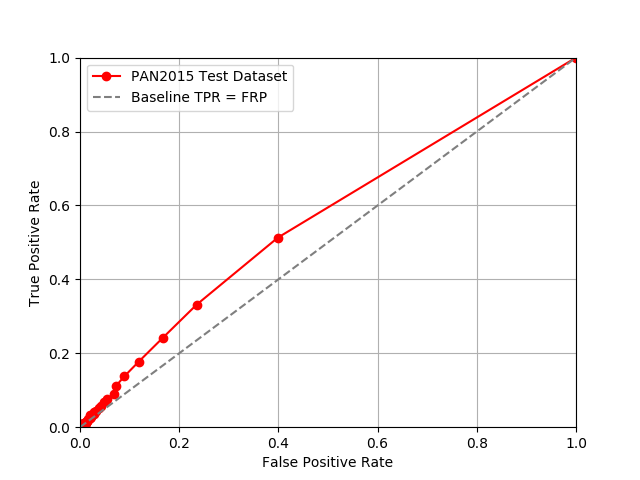
\includegraphics[width=.7\textwidth]{./pictures/delta_method_roc.png}
    \caption{The ROC curve of the delta method with number of opposing authors
    varying from 0 to 10 using the two test datasets for PAN2013 and the test
    dataset for PAN2015.}
    \label{fig:delta_method_roc}
\end{figure}

\subsection{Generalizing Random Forest}
After creating our \gls{UBM} based on the training data, we got the following results on the test 
data, after training our random forest using the two different encondings presented.

\begin{align}
\text{UBM Enconding Accuracy}:&\qquad 0.616\\
\text{Subtraction Enconding Accuracy}:& \qquad 0.604
\end{align}

\subsection{Extended Delta}

\subsection{Author Specific SVM}
% SVM performs well on binary authorship problems Abbasi & Chen, 2008; Zheng et al., 2006
% from https://pdfs.semanticscholar.org/5c2b/6876df693e096c6c150a5b0d2a2c05043003.pdf
